\documentclass{suribt}
\title{ゲーム「2048」のプレイヤについて}
\author{金澤望生}
\eauthor{Kanazawa Nozomu}
\studentid{08-152021}
\supervisor{山口和紀 教授}
\handin{2018}{1}
\keywords{ゲームAI,機械学習}
\usepackage[dvipdfmx]{graphicx}
\usepackage{float}

\begin{document}
\maketitle

\frontmatter
\begin{abstract}
インターネットブラウザやスマートフォン上で遊ぶことのできるパズルゲーム「2048」をプレイするAIの改良を行った.改良には盤面上で最も大きな数のタイルが隅にあることを重視する独自のヒューリスティック「corner bonus」を使用した.(仮)
\end{abstract}

\tableofcontents

\mainmatter
\chapter{導入}
モチベーションや2048の基本ルール・指標について説明します.

\chapter{先行研究の紹介}
既存研究が使用している手法とプレイヤの成績について説明します.

\section{Szubert \& Jaskowski (2014)}
Szubert \& Jaskowskiは,TD学習を用いたプレイヤの訓練とnタプルネットワークを用いた価値関数の表現を組み合わせることによって,人間の知識やゲーム木探索を使用しないで十分強い2048プレイヤを実装することに成功した。
\subsection{TD学習}
TD学習の「TD」とはtemporal differenceの略であり,すなわち状態間における価値の差分を学習することによって学習器の訓練を行う手法である。2048にあてはめると,とある盤面$s'$の価値と,その盤面の1プレイ後の盤面$s'_{next}$の価値の差分を取り,これを現状定まっている$s'$に足し込んでいくことで訓練を行うことになる。TD学習にはさまざまな派生があるが,Szubert \& Jaskowskiが使用しているTD(0)学習は以下の式によって表現される:

\[
	V(s) ← V(s) + \alpha (r + V(s'') - V(s) )
\]

この式において,$V$は価値関数,$\alpha$は学習率,$r$は報酬である。学習率は計算された差分を価値関数の更新にどれほど反映するかを決定するパラメータである。

TD学習はTesauroによるバックギャモンへの適用でよく知られるようになり,碁やオセロ,チェスにおけるゲームAIの方策決定の手法として用いられるようになった。

\subsection{nタプルネットワーク}
TD学習によって盤面の評価とその学習を行うことができるが,盤面と評価値をどのように結びつけるかが問題になる。まず,2048で有り得るすべての盤面に対して評価値を与える1対1対応のルックアップテーブル(LUT)を作成することを考えると,2048で有り得る盤面の数は$(4 \times 4)^{18} \approx 4.7 \times 10^{21}$と膨大な数になり,このようなLUTを計算機上で実装することは現実的に不可能である。

そこで,一部のマスの組み合わせによる「タプル」というクラスターを作成し,さらに複数のタプルを組み合わせることで盤面を表現する手法「nタプルネットワーク」を2048に導入することが,Szubert \& Jaskowskiによって提案された。たとえば,下記のようなnタプルネットワークを実装した場合,1つのゲーム内で保持すべき重みの数は860625であり,全ての有り得る盤面に対するLUTを保持するのに対して非常に少なくて済む。

\begin{figure}[H]
	\centering
	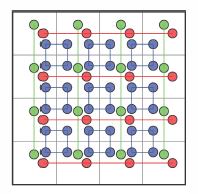
\includegraphics[width=5cm]{figure_001.png}
	\caption{nタプルネットワークの例}
\end{figure}

nタプルネットワークはBledsoe \& Browning (1959)によりパターン認識に用いられたのが最初の採用例である。ゲームAIの分野ではJaskowski (2014)によってオセロに適用され,一定の成果が得られた。

\subsection{結果と課題}
本手法をもとに行った実験のうち,最も良い勝率を達成したプレイヤを用いて10万ゲーム中の成績を検証したところ,勝率は0.9781であり,平均スコアは100,178であった.1ゲーム中に達成されたスコアで最も良かったのは261,526であった.Szubert \& Jaskowskiによる新たな手法は探索ベースの手法よりも大幅に高速で,かつ成績が良かった.

しかしながら,この手法では「常に2048-tileを生成すること」よりも「時々16384-tileを生成すること」を重視しているため,勝率は必ずしも100\%を達成できていない.また,人間の知識を一切導入していないため,最も大きな数のタイルが盤面上の端に配置されないなど,人間の直感的な戦略とは反しているといったデメリットがあった.

\section{Wu et al. (2014)}
Wuは,Szubert \& Jaskowskiの手法を改良し,木探索を用いた先読みと組み合わせることによってさらに良いプレイヤを実装することに成功した.
\subsection{nタプルネットワークの配置の改善}
Wuは,Szubert \& Jaskowskiが考案したnタプルネットワークのうち,直線型で4タプルとして配置していたタプルを,図2.2.(b)のように柄杓型の6タプルに変更した.これによって増える重みの数は約2倍程度であったが,この変更によってSzubert \& Jaskowskiのものよりも飛躍的に良い成績を得ることができた.なお,なぜこのようなタプルの配置が最善だと判断したのかについて,Wuは論文において言及していない.

\begin{figure}[H]
	\centering
	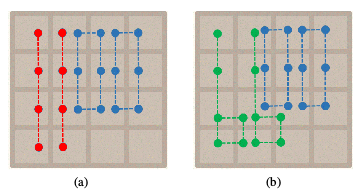
\includegraphics[width=8cm]{figure_002.png}
	\caption{Szubert \& Jaskowski(a)とWu(b)が提唱したnタプルネットワーク}
\end{figure}

\subsection{Multi-Stage TD学習の導入}
Multi-Stage TD学習(MS-TD学習)とは,ゲームの局面に応じて異なる価値関数を保持することによって,よりそれぞれの局面に対して適切な重みを学習させることを目的とした手法である.Wuは学習のプロセスを3つのステージに分割し,ゲームプレイも同様に3つのステージに分割して行うようにした.Wuの提唱した2048におけるMS-TD学習は,以下のような手順で学習を行う.なお,「$T_{16k}$」とは「そのゲーム中で初めて16384-tileを生成することに成功した時」,「$T_{16+8k}$」とは「そのゲーム中で初めて16384-tileを生成した後に,初めて8192-tileを生成することに成功した時」のことを示す.

\begin{enumerate}
\item 第1ステージにおいては,初期盤面からゲームを始めて,価値関数が十分飽和するまで学習を行う.このステージで学習された価値関数の重みのことを「Stage-1価値関数」と呼ぶことにする.また,学習ゲーム中に$T_{16k}$を達成したなら,その時の盤面を全て保存しておく.
\item 第2ステージにおいては,第1ステージで保存した盤面からゲームを始めて,TD学習を行う.このステージで学習された価値関数の重みのことを「Stage-2価値関数」と呼ぶことにする.また,学習ゲーム中に$T_{16+8k}$を達成したなら,その時の盤面を全て保存しておく.
\item 第3ステージにおいては,第2ステージで保存した盤面からゲームを始めて,TD学習を行う.このステージで学習された価値関数の重みのことを「Stage-3価値関数
」と呼ぶことにする.
\end{enumerate}

その後,以下のような手順でゲームプレイを行う.

\begin{enumerate}
\item 盤面が$T_{16k}$を達成するまでは,Stage-1価値関数を用いてゲームプレイを行う.
\item 盤面が$T_{16k}$を達成してから$T_{16+8k}$を達成するまでは,Stage-2価値関数を用いてゲームプレイを行う.
\item 盤面が$T_{16+8k}$を達成してからは,Stage-3価値関数を用いてゲームプレイを行う.
\end{enumerate}

\subsection{Expectimax木探索}
Szubert \& Jaskowski (2014)によって,木探索ベースの2048プレイヤは強化学習で訓練したプレイヤに劣ることが示されたが,Wuは強化学習によるプレイヤに対してExpectimax木探索を補助的に組み合わせることによって,さらにプレイヤの性能を高めようと試みた.

\begin{figure}[H]
	\centering
	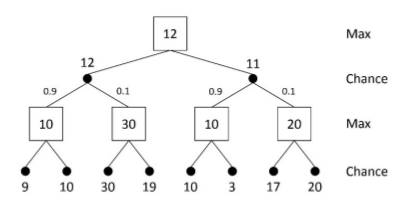
\includegraphics[width=8cm]{figure_003.png}
	\caption{Expectimax木の例 (Wu et al. (2015))}
\end{figure}

Expectimax木探索には,MaxノードとChanceノードという2種類のノードがあり,それぞれのノードの値は子ノードから決定される.Maxノードの値は,子ノードのうち最も大きな値のノードの値となる.例えば図2.3.の根ノードの値は12であるが,これは子ノードの「12」と「11」のうち最大の値である12を取ったものである.一方でChanceノードの値は子ノードの期待値となる.例えば図2.3.の根ノードの子ノードの1つである「12」というノードは,0.9の確率で10となるノードと0.1の確率で3となるノードの期待値,すなわち$0.9 \times 10 + 0.1 \times 3 = 12$によって12という値が決定する.

Wuの提案においては,Maxノードの値はプレイヤがアクションを選択して遷移を行った後の盤面,Chanceノードは遷移を行った後にランダムタイルを発生させた後の盤面が与える評価値となる.例えば,ある盤面$s$(アクション選択と遷移が終わった直後の盤面とする)の評価値を深さ3のExpectimax木探索を用いて求めたい時,図2.4.のような探索木が考えられる.$s$の盤面が分かれば,その子ノードであるランダムタイル生成後の盤面,さらにその子ノードである遷移後の盤面を求めることができる.さらに,葉ノードにあたるChanceノードの値は価値関数が与える評価値とすることで,各ノードの値を求めることができ,最終的に根ノード,すなわち評価値を求めたい盤面$s$の評価値も求められるということになる.

(図2.4. 何かいい感じの2048の探索木を自分で描画して貼る)

\subsection{結果と課題}
WuによるプレイヤはSzubert \& Jaskowskiのものに比べて著しく良い成績を達成した.まずSzubert \& Jaskowskiが達成できなかった32768-tileの生成に成功し,10.9\%の確率で32768-tileを生成できるようになった.勝率に関しては1を達成,すなわち2048-tileは100\%の確率で生成できるようになり,平均スコアは328,946,最大スコアは605,752を記録した.これは当時としては1つの例外\footnote{Xiaoによる深深度先読みと人間による調整を行った評価関数を用いたプレイヤがこれにあたるが,Wuのものよりも100倍遅い:https://www.youtube.com/watch?v=JQut67u8LIg}を除き,計算機による2048プレイヤの中で最も優れた成績であった.

一方で,nタプルネットワークの形状変更やMS-TD学習のステージングについては,この研究で行なわれた調整についてこれといった根拠が述べられておらず,依然として改良の余地は残していた.特にnタプルネットワークの形状変更については,次のOka \& Matsuzakiの研究で詳しく検討されることとなった.

\chapter{本研究のアイディア}
本研究で導入しようとしている手法のアイディアについて説明します.

\chapter{提案と実装}
前章で説明したアイディアの具体的な提案とその実装方法を説明します.

\chapter{実験}
提案したアイディアの実験結果と既存研究の実験結果を比較します.

\chapter{考察と結論}
実験結果をもとに,結果の考察を行い,本研究をまとめます.

\backmatter
\chapter{謝辞}
謝辞を書きます.

\begin{thebibliography}{}
 \bibitem{}
 \bibitem{}
\end{thebibliography}

\appendix
\chapter{}
表やプログラムリストの掲載が必要になったらここに掲載します.

\end{document}
